\documentclass{article}

\usepackage[a4paper, total={6.5in, 11in}]{geometry}
\usepackage{graphicx}
\usepackage{subfig}
\usepackage{gensymb}
\graphicspath{{titech/CSC.T463.ComputerGraphics/h4/}}

\usepackage{latex/common}

\title{Computer Graphics 2021 - Assignment 4}
\author{Sixue Wang\\21M30927\\Tokyo Institute of Technology}

\begin{document}

\maketitle

\section*{Equation}
The basic idea is use translation(mats.glTranslatef) to imitate revolution and use rotation(mats.glRotatef) to imitate rotation.
We suppose Sun is fixed,
orbits of Earth and Moon are static ellipses,
and speeds of Earth and Moon revolution are constant.
The animation is determined by the angle of Earth revolution $t$.
In OpenGL, x-axis is horizontal, y-axis is vertical and z-axis is depth.
We don't need to care about perspective projection because OpenGL will handle it automatically.
For easier observation, we adjust the speed of Earth rotation, sizes of Earth and Moon, and distances among Sun, Earth, and Moon.

\subsection*{Sun}
The position of Sun is fixed but we want to put it far away from the screen so everything can fit in a small window.
\begin{equation}
  \begin{bmatrix}
    1 & 0 & 0 & 0     \\
    0 & 1 & 0 & 0     \\
    0 & 0 & 1 & -18   \\
    0 & 0 & 0 & 1
  \end{bmatrix}
\end{equation}
For Sun rotation, we need calculate the angle at first:
\begin{equation}
  solar\_t = t * \frac{EARTH \; ORBITAL \; PERIOD}{SOLAR \; ROTATION \; PERIOD} = t * \frac{365}{24.47}
\end{equation}
To be simple, we assume the obliquity of Sun rotation is $0^{\circ}$, so it rotates along $[0, 1, 0]$:
\begin{equation}
  \begin{bmatrix}
    cos(solar\_t) & 0 & sin(solar\_t) & 0   \\
    0 & 1 & 0 & 0   \\
    -sin(solar\_t) & 0 & cos(solar\_t) & 0   \\
    0 & 0 & 0 & 1
  \end{bmatrix}
\end{equation}

\subsection*{Earth}
The position of Earth is:
\begin{equation}
  \begin{bmatrix}
    1 & 0 & 0 & x = EARTH \; ORBITAL \; A * cos(-t)          \\
    0 & 1 & 0 & tan(EARTH \; ORBITAL \; INCLINATION * x)     \\
    0 & 0 & 1 & EARTH \; ORBITAL \; B * sin(-t)              \\
    0 & 0 & 0 & 1
  \end{bmatrix}
\end{equation}
The angle of Earth rotation is:
\begin{equation}
  earth\_t = t * \frac{EARTH \; ORBITAL \; PERIOD}{EARTH \; ROTATION \; PERIOD} = t * 365
\end{equation}
And it rotates along $[tan(EARTH \; OBLIQUITY), 1, 0]$:
\begin{equation}
  r_x = \frac{tan(EARTH \; OBLIQUITY)}{1+tan(EARTH \; OBLIQUITY)^2} \\
\end{equation}
\begin{equation}
  r_y = \frac{1}{1+tan(EARTH \; OBLIQUITY)^2} \\
\end{equation}
\begin{equation}
  \begin{bmatrix}
    cos(earth\_t)+(1-cos(earth\_t))r_x^2 & (1-cos(earth\_t))r_xr_y & r_ysin(earth\_t) & 0   \\
    (1-cos(earth\_t))r_xr_y & cos(earth\_t)+(1-cos(earth\_t))r_y^2 & -r_xsin(earth\_t) & 0   \\
    -r_ysin(earth\_t) & r_xsin(earth\_t) & cos(earth\_t) & 0   \\
    0 & 0 & 0 & 1
  \end{bmatrix}
\end{equation}
Then we resize Earth with:
\begin{equation}
  \begin{bmatrix}
    \frac{EARTH \; SIZE}{SUN \; SIZE} & 0 & 0 & 0          \\
    0 & \frac{EARTH \; SIZE}{SUN \; SIZE} & 0 & 0     \\
    0 & 0 & \frac{EARTH \; SIZE}{SUN \; SIZE} & 0              \\
    0 & 0 & 0 & 1
  \end{bmatrix}
\end{equation}

\subsection*{Moon}
The angle of Moon revolution is $moon\_t = t * \frac{EARTH \; ORBITAL \; PERIOD}{MOON \; ORBITAL \; PERIOD}$
The position of Moon is:
\begin{equation}
  \begin{bmatrix}
    1 & 0 & 0 & EARTH \; ORBITAL \; A * cos(-t) +  MOON \; ORBITAL \; A * cos(-moon_t)         \\
    0 & 1 & 0 & tan(EARTH \; ORBITAL \; INCLINATION * EARTH \; ORBITAL \; A * cos(-t))     \\
    0 & 0 & 1 & EARTH \; ORBITAL \; B * sin(-t)  +  MOON \; ORBITAL \; B * sin(-moon_t)          \\
    0 & 0 & 0 & 1
  \end{bmatrix}
\end{equation}
The angle of Moon rotation is $moon\_t = t * \frac{EARTH \; ORBITAL \; PERIOD}{MOON \; ROTATION \; PERIOD}$
To be simple, we assume the obliquity of Moon rotation is $0^{\circ}$, so it rotates along $[0, 1, 0]$:
\begin{equation}
  \begin{bmatrix}
    cos(moon\_t) & 0 & sin(moon\_t) & 0   \\
    0 & 1 & 0 & 0   \\
    -sin(moon\_t) & 0 & cos(moon\_t) & 0   \\
    0 & 0 & 0 & 1
  \end{bmatrix}
\end{equation}
Then we resize it.

\section*{Instruction}
I just modified ``display'' function in the ``SimpleRotation.java''. So you can build the program by ``make'' as before.


\section*{Result}

I also attached a screen record named ``animation.mp4'' under the root directory ``SimpleExample2021''.

\begin{figure}[h]
  \begin{tabular}{cc}
    \subfloat[]{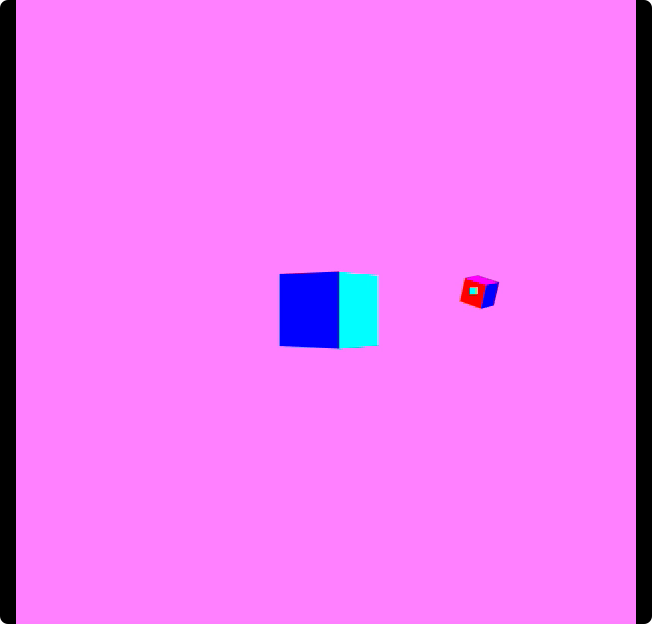
\includegraphics[width=0.3\textwidth]{h4_1.png}} &
    \subfloat[]{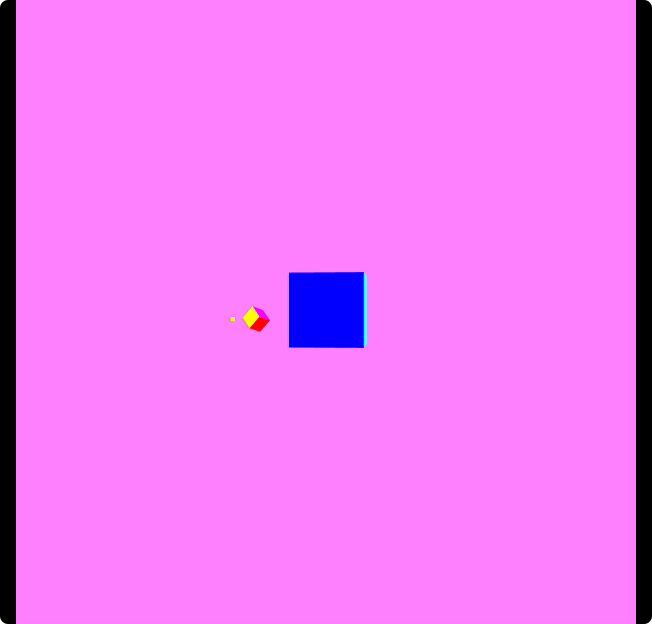
\includegraphics[width=0.3\textwidth]{h4_3.png}} \\
    \subfloat[]{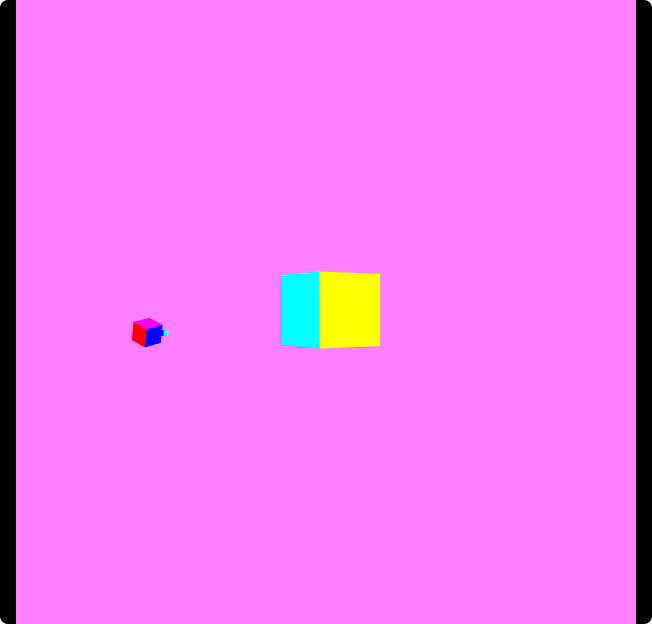
\includegraphics[width=0.3\textwidth]{h4_4.png}} &
    \subfloat[]{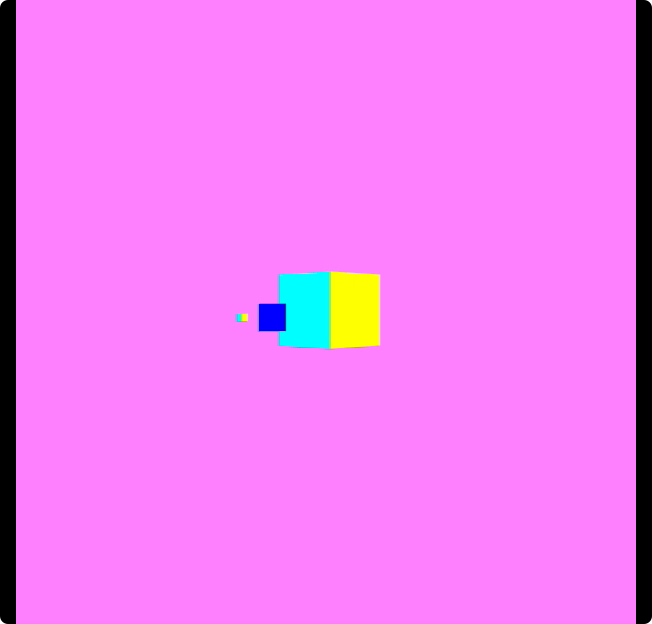
\includegraphics[width=0.3\textwidth]{h4_5.png}} \\
    \subfloat[]{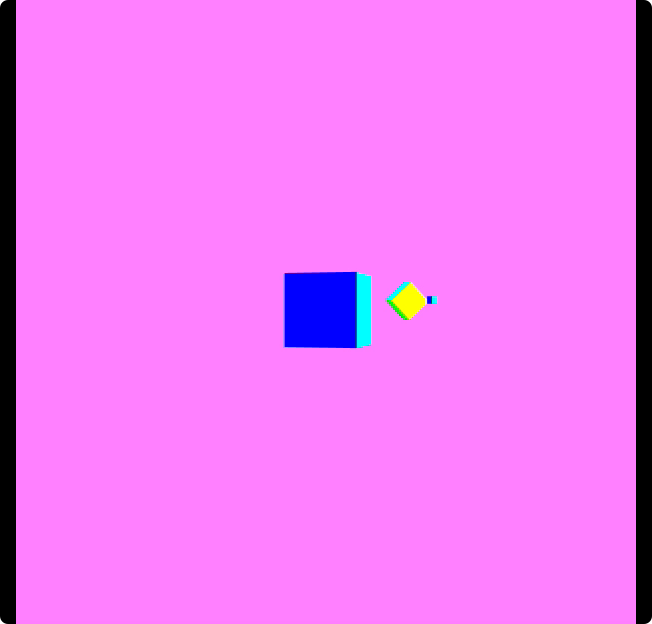
\includegraphics[width=0.3\textwidth]{h4_6.png}} \\
  \end{tabular}
\end{figure}


\end{document}
